\mnDifficult
\begin{slikaDesno}{fig/mot_step.pdf}[fig/mot_blok.pdf]
\PID
Мотор за једносмерну струју се може моделовати функцијом преноса у облику $M(s) = \dfrac{K_0}{s\uptau + 1}$, где 
су $K_0$ и $\uptau$ непознате константе. Улаз тог система 
сигнал $v = v(t)$ који представља напон на прикључцима мотора, а његов излаз је обртна брзина вратила тог мотора 
$w = w(t)$. \\[1mm]
\begin{enumerate}[label=(\alph*)] 
    \itemsep1pt
    \item Када се на мотор доведе побуда у облику
    $v(t) = V_0 \uu(t)$, $V_0 = 10\unit{V}$, одзив је прецизно уцртан на 
    графику датом на слици 1.1. 
    Проценити напознате коефицијенте 
    $K_0$ и $\uptau$. Инжењерске апроксимације су дозвољене. 
    За обртну брзину задржати јединицу обртаја у минути 
    $\rm[rpm]$. 
\end{enumerate}
\end{slikaDesno}
\begin{enumerate}[label=(\alph*)]\refstepcounter{enumi}
    \item Испред мотора се каскадно везује 
    управљачки систем $G(s)$ (по природи, напонски
    појачавач), као на слици 1.2. 
    Одредити $G(s)$ тако да одзив целог система 
    на побуду $u(t) = V_0\uu(t)$, $V_0 = 10\unit{V}$,
    буде дупло бржи него у претходној тачки 
    $w^{\text{(б)}}(t) =  w^{\text{(а)}}(2t)$. 
    \item 
    За случај из претходне тачке, 
    скицирати временски дијаграм сигнала $v(t)$. 
    \item 
    Реализовати напонски појачавач чија је фунцкија преноса $G(s)$ помоћу једног 
    идеалног операционог појачавача са произвољним бројем пасивних елемената у колу. 
    Излаз појачавача може бити и инвертован. 
\end{enumerate}

\RESENJE

(а) Да би се одредили тражени коефицијенти, потребно је изразити дати одзив у зависности од њих. Односно, потребно 
је одредити општи облик одзива $w(t)$. 
Лапласова трансформација одзива на побуду одређује се множењем Лапласове трансформације побуде са 
функцијом преноса система у $s$-домену. Према табличном резултату \reft{T:LT:u} је онда 
\begin{equation}
    W(s) = \underbrace{V(s)}_{\LT{v(t)}} M(s) = M(s) = \dfrac{V_0 K_0}{s(s\uptau + 1)}.
\end{equation}
Одговарајући одзив у временском домену одређује се одређивањем инверзне Лапласове трансформације. У овом случају, 
то се може урадити растављањем на парцијалне разломке 
$\dfrac{V_0 K_0}{s(s\uptau + 1)} = \dfrac{A}{s} + \dfrac{B}{s\uptau + 1}$, 
како је описано 
у додатку \ref{a:pfd},
\begin{eqnarray}
    && A = \dfrac{V_0 K_0}{\xcancel s (s\uptau + 1)} \Bigg|_{s = 0} = V_0 K_0, \qquad 
    B = \dfrac{V_0 K_0}{ s \xcancel{(s\uptau + 1)}} \Bigg|_{s = -1/\uptau} = -\uptau 
    V_0 K_0.
\end{eqnarray}
Применом своства линеарности, и одговарајућих табличних трансформација, се онда одређује одзив у временском 
домену
\begin{equation}
    w(t) = \ILT{W(s)} = K_0 V_0 \underbrace{\ILT{ \dfrac{1}{s} }}_{\text{ \reft{T:LT:u} } : \uu(t)} 
    - K_0 V_0 \underbrace{\ILT{\dfrac{1}{s + \uptau^{-1}}}}_{\text{ \reft{T:LT:exp} } : \ee^{-t/\uptau} \uu(t) }
    = K_0 V_0 (1 - \ee^{-t/\uptau}) \uu(t) \label{eq:\ID.oblik}
\end{equation}
Одавде се тражени коефицијент са графика могу прочитати на различите начине. У овом случају коефицијент $K_0$ се 
може одредити разматрањем практично устаљеног стања, односно $w(\infty) \to K_0 V_0$. Са датог дијаграма може  
се установити да је $w(\infty) \approx 3000\unit{rpm}$ тако да је $K_0 \approx 3000\unit{rpm}/V_0$, односно је 
\begin{eqnarray}
    K_0 \approx 300\unit{\dfrac{rpm}{V}}.
\end{eqnarray}
За одређивање другог коефицијента, са графика са може проценити једна тачка 
$w(t = T)$, на основу чега се може одредити непозната временска константа
решавањем по њој из израза \eqref{eq:\ID.oblik},
\begin{eqnarray}
    w(T) = K_0V_0(1 - \ee^{-T/\uptau}) \cancelto{1}{\uu(T)} \Rightarrow
    \uptau = \dfrac{T}{
        \ln \dfrac{1}{1 - \dfrac{w(T)}{K_0 V_0}}.
    }
\end{eqnarray}
Одабир времена $T$ теоријски је прозивољан, међутим, пошто постоји дељење са 
$1 - \dfrac{w(T)}{K_0 V_0}$, резултат ће бити веома непрецизан ако се одабере $\dfrac{w(T)}{K_0 V_0} \approx 1$. Другим речима, 
потребно је одабрати неки од тренутака где је прелазни процес изражен, знатно пре успостављања стационарног стања. 
На пример, одабиром $T = 2\unit{s}$, на основу чега се израчунава\footnote{Тачне вредности параматара 
са којима је график нацртан су $K_0 = 300\unit{rpm/V}$ и $\uptau = 2\unit{s}$} $\uptau \approx 1,8\unit{s}$. 

(б) Мотивисано поступком из претходне тачке, односно изразом \eqref{eq:\ID.oblik} треба одзив треба да буде 
\begin{equation}
    w^{\text{(б)}}(t) = w^{\text{(а)}}(2t) = 
    K_0 V_0 (1 - \ee^{-2t/\uptau}) \uu(t) 
    =
    K_0 V_0 (1 - \ee^{-t/ \overbrace{\uptau/2}^{\uptau'} }) \uu(t).
\end{equation}
Односно, временска константа система у целини треба да буде $\uptau' = \dfrac{\uptau}{2}$. 
Односно, преносана функција целог система треба да буде иста као и $M(s)$, са другом временском константом. Односно је 
\begin{eqnarray}
    G(s)M(s) = \dfrac{K_0}{s\uptau' + 1} = G(s) \cdot \dfrac{K_0}{s\uptau' + 1}
    \Rightarrow 
    G(s) = \dfrac{  
        \dfrac{\cancel{K_0}}{s\uptau' + 1}
     }{ 
        \dfrac{\cancel{K_0}}{s\uptau + 1}
     }
     =
     \dfrac{s\uptau + 1}{s\uptau' + 1}.
\end{eqnarray}
Односно, систем $G(s)$ треба да уведе нулу функције преноса која „поништава“ пол постојеће функције преноса $M(s)$, 
и додаје нови дупло бржи пол. 


\begin{figure}[b!]
    \centering
    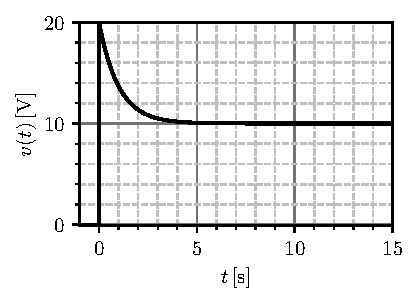
\includegraphics[]{fig/mot_os.pdf}
    \caption{Уз резултат задатака.}
    \label{fig:\ID.os}
\end{figure}


(в) Временски дијаграм сигнала $v(t)$ одређује се одређивањем одзива система $G(s)$ на задату побуду, поступком 
сличним као у тачки (а), па је 
\begin{equation}
    V(s) = G(s) U(s) = \dfrac{V_0 (s + \uptau)}{s (s\uptau' + 1) } = 
    \dfrac{A}{s} + \dfrac{B}{(s + \uptau')} \label{eq:\ID.vs}
\end{equation}
Коефицијенти развоја у парцијалне разломке су 
\begin{equation}
    A =  \dfrac{V_0 {(s\uptau + 1)}}{\xcancel s (s\uptau' + 1) } \Bigg|_{s = 0} = V_0 \\
    B =  \dfrac{V_0 {(s\uptau + 1)}}{ s \xcancel{(s\uptau' + 1)} } \Bigg|_{s = -1/\uptau'}
    = \uptau' V_0 \left(\dfrac{\uptau}{\uptau'} - 1\right)
\end{equation} 
Заменом коефицијената у израз \eqref{eq:\ID.vs}, па табличним одређивањем инверзне Лапласове трансформације добија се 
\begin{eqnarray}
    v(t) &=& \ILT{V(s)} 
    = V_0 \underbrace{\ILT{ \dfrac{1}{s} }}_{\text{ \reft{T:LT:u} } : \uu(t)}  + V_0\left( 
        \dfrac{\uptau}{\uptau'} - 1
     \right)
     \underbrace{\ILT{
        \dfrac{1}{s + (\uptau')^{-1} }
     }}_{\text{ \reft{T:LT:exp} } : \ee^{-t/\uptau'} \uu(t)} 
     \\
     &=& 
    V_0 \uu(t) +  V_0\left( 
        \dfrac{\uptau}{\uptau'} - 1
     \right) \ee^{-t/\uptau'}
     \uu(t).
     = 
     V_0\uu(t) 
     + 
     V_0 \ee^{-t/\uptau'}
\end{eqnarray}

Прокоментаришимо добијени резултат. Први члан у изразу одговара улазном напону, односно, то је практично 
улаз прошуштен до излаза. Са друге стране, други сабирак даје краткотрајно улазни напон већи од оног 
потребног да би систем брже успоставио коначно стање. Ово јесте основ оваквог механизма убрзавња одзива
система, који услед 
постојања нуле функције преноса у левој комплексној полуравни има тзв. \textit{прескок} у тренутку дејства побуде. 
График добијеног резултата приказан је на слици \ref{fig:\ID.os}. 

\begin{wrapfigure}{r}{0.3\textwidth}
    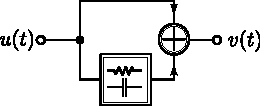
\includegraphics[page=1]{fig/mot_kolo.pdf}  
    \caption{Идеја за реализацију.}  
    \label{fig:\ID.blok}
\end{wrapfigure}
(г)
Коло се може пројектовати користећи се аргументима из претходне тачке. Структурно, тражени систем 
реализује се као систем чији блок дијаграм илустрован на слици \ref{fig:\ID.blok}. 
Коло са отпорником и кондензатором треба да реализује временску константу 
$\uptau' \approx 1\unit s$, и да се излаз тог кола сабере са улазом. Сабирање напона може 
се извести \textit{инвертујућим сабирачем} са операционим појачавачем, будући да је по услову
задатка дозвољено да излаз буде инвертован. На слици \ref{fig:\ID.kolo} је приказано тако Мотивисано
коло. Кондензатор $C_{\rm F}$ и отпорник $R_{\rm F}$ реализују ВФ филтар чија временска константа 
треба да буде $\uptau'$, док инвертујући сабирач на излаз филтра још једном сабира улаз. Да сабирач 
не би утицао на рад филтра, потребно је да је отпорност која се види десно од филтра буде много 
већа од отпорника у филтру, $R \gg R_{\rm F}$. Уколико усвојимо разуман највећи ред величина 
за отпорнике $\sim 100\unit{k\Omega}$, могу се одабрати вредности 
$C_{\rm F} = 500\unit{\upmu F}$, $R_{\rm F} = 2\unit{k\Omega}$, и 
$R_{\rm F} = 200\unit{k\Omega}$. 

\begin{figure}[ht!]
    \centering 
    \includegraphics[page=2]{fig/mot_kolo.pdf}        
    \caption{Реализација појачавача $G(s)$.}
    \label{fig:\ID.kolo}
\end{figure}

Алтернативно, могуће је приметити и да је отпорник $R_{\rm F}$, тополошки паралелно везан отпонику 
$R$ са којим дели један заједнички крај (јер је због постојања операционог појачавача напон инвертујућег
улаза једнак нули). 
Тиме је тачна временска константа датог филтра заправо $C_{\rm F} (R_{\rm F} \parallel R)$, па би било
могуће одабрати и $C_{\rm F} = 10\unit{\upmu F}$, $R_{\rm F} = R = 200\unit{k\Omega}$.  Ово је повољнији 
дизајн, јер уместо занемаривања он \textit{користи} улазну отпорност наредног степена, чиме се постиже 
већа слобода у избору параметара -- и из тог разлога и бољи дизајн.
